%!TEX root = index.tex
\chapter[Metodologia]{Metodologia}
\label{chap:metodologia}
Nesse capítulo será apresentado o método utilizado para o desenvolvimento do estudo que visa a tentativa de salvar a empresa Beeconnect. De acordo com a introdução realizada no Capítulo 1, a Beeconnect estava prestes a ser encerrada pelo Conselho da holding Techmob. Entre os motivos estavam: o fato da empresa estar gastando muito em recursos humanos, quase quinhentos mil reais no decorrer de um ano, e o fato da startup ainda não ter provado o seu modelo de negócio. Mesmo após meses e meses de trabalho árduo nenhum varejista ainda estava disposto a pagar pelo serviço oferecido pelo aplicativo.

Conforme explicado nos Objetivos do trabalho de formatura, a intenção é provar que empresa possui um modelo de negócio que gera valor para os seus clientes e que seja sustentável, ou seja, os varejistas devem estar dispostos a pagar pelo serviço e ao mesmo tempo deve haver sobrar uma margem de lucro positiva. Foram utilizados os conceitos apresentados na revisão bibliográfica, principalmente os textos elaborados por \citeonline{leanstartup}, \citeonline{startupowners} e \citeonline{businessmodel}.

A metodologia utilizada nesse trabalho de conclusão de curso foi dividida nos seguintes tópicos e ilustrada na \autoref{fig:metodologia}:
\begin{enumerate}
\item Mapear estado atual da startup
\item Gerar hipóteses sobre a proposta de valor da empresa.
\item Desenhar os testes de hipóteses.
\item Testar hipóteses.
\item Analisar resultados e repetir o ciclo.
\item Listar lições aprendidas.
\end{enumerate}

\begin{figure}[H]
\caption{Metodologia utilizada}
\centerline{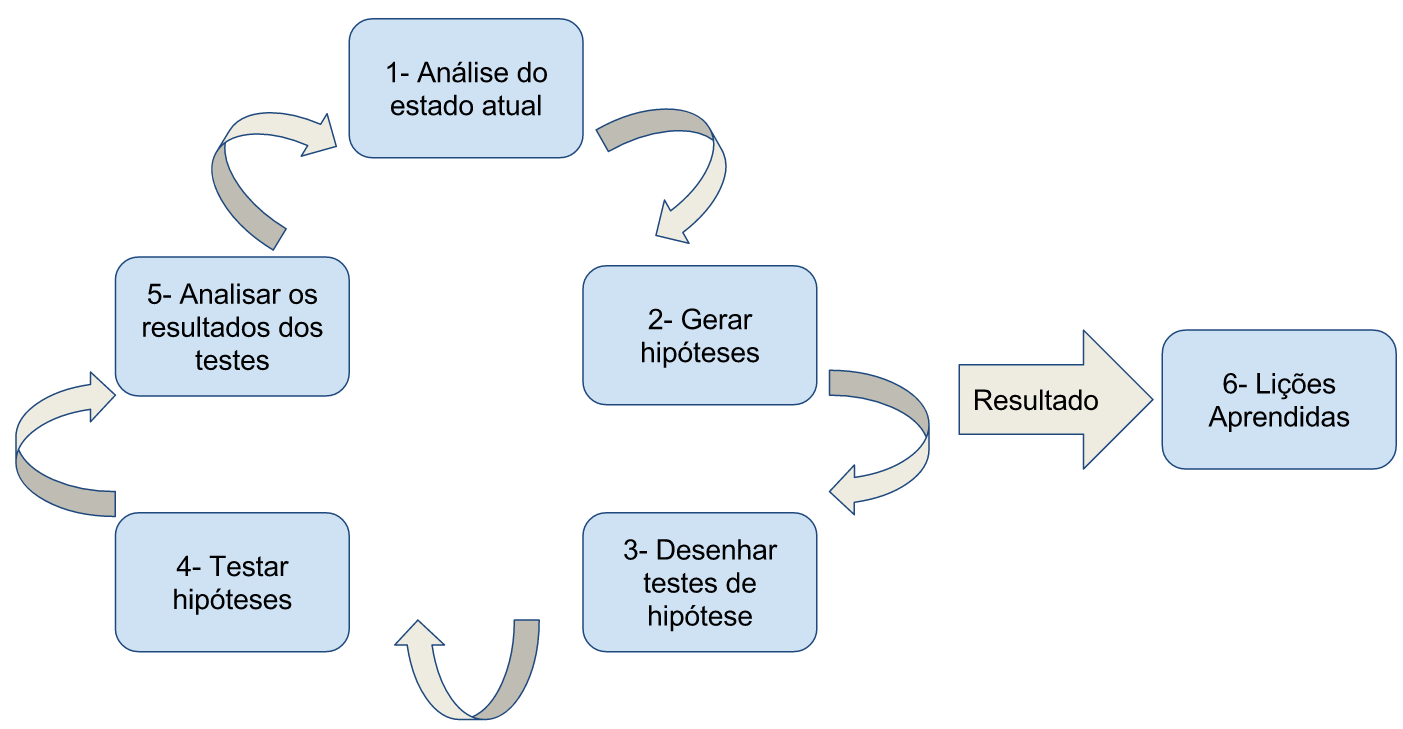
\includegraphics[scale=0.25]{img/metodologia}}
\label{fig:metodologia}
\caption* {Fonte: Elaborado pelo autor}
\end{figure}

\section{Mapear estado atual da startup}
\label{cha:mapear_estado}
Para mapear o estado atual da startup baseado no aplicativo Beeconnect foi utilizado o conceito do Canvas de Modelo de Negócio apresentado por \citeonline{businessmodel}.
O autor contou com a ajuda dos demais membros da Beeconnect para elaborar no escritório da empresa um canvas de modelo de negócio, preenchendo cada um dos nove blocos de modo a permitir uma melhor visualização e compreensão do estado atual da empresa na época. 

Conforme recomendado por  \citeonline{businessmodel}, foram utilizados \textit{post-its} que ficaram grudados em uma lousa o que facilitou muito as alterações, assim foram feitas diversas iterações até que finalmente chegou-se em um modelo que agradou a todos. Depois, o autor passou o modelo para o \textit{Google Docs} para que todos tivessem fácil acesso ao Canvas, e que também permitiu o compartilhamento de tal modelo com o professor André Fleury.

\section{Gerar hipóteses sobre a proposta de valor da empresa}
\label{cha:gerar_hipoteses}
Para gerar as hipóteses sobre a proposta de valor da empresa foram utilizados os conceitos de Validação do Cliente de \citeonline{startupowners}, o capítulo de Experimentação de Startups de \citeonline{leanstartup}, e os conceitos propostos por \citeonline{businessmodel} e \citeonline{valueproposition}.    

Uma vez que o Canvas de Modelo de Negócio da Beeconnect estivesse pronto o autor reuniu-se com o professor André Fleury na Escola Politécnica para gerar as hipóteses sobre a proposta de valor da empresa. Tais suposições conectaram os blocos Segmentos de Clientes e Proposição de Valor.

\section{Desenhar os testes de hipóteses}
\label{cha:desenhar_hipoteses}
Após gerar as hipóteses o autor também recorreu a mentoria do professor André Fleury para que os testes realmente testassem as hipóteses. Juntos os dois desenharam os testes e as métricas que definiriam se a Beeconnect passou ou não no teste. 
Além disso o autor reuniu-se com sua equipe para planejar como os testes seriam implementados. A equipe respondeu as perguntas abaixo para cada teste:
\begin{itemize}
\item Quando o teste será realizado?
\item Quem realizará o teste?
\item Onde o teste será executado?
\item Quanto custaria para realizar o teste?
\item Quanto tempo levaria para realizá-lo?
\end{itemize}

\section{Testar hipóteses}
\label{cha:testar_hipoteses}
Após planejar como realizar cada teste com o intuito de testar as hipóteses de valor, a equipe da Beeconnect foi a campo responder cada uma das suposições geradas. Basicamente, foi a aplicação do conceito do \textit{Genchi Genbutsu} de "saia e veja por si mesmo" utilizado na manufatura enxuta e mencionado por \citeonline{leanstartup}.

Os membros que foram a campo deveriam levar um caderno para que anotassem os aprendizados para depois compartilhar com os demais integrantes da empresa. Por exemplo anotar as reações dos varejistas quando expostos a diferentes preços do serviço, ou quais dúvidas que os usuários poderiam ter a respeito do aplicativo.

\section{Analisar resultados e repetir ciclo}
\label{cha:analisar_resultados}
Uma vez que os testes foram realizados e os resultados obtidos o autor checou se a Beeconnect passou ou não nos testes, ou seja, se as hipóteses foram provadas ou se foram refutadas. 
Após tal análise o autor reuniu-se novamente com o professor André Fleury para que juntos eles iterassem novamente pelo ciclo de modo que mais hipóteses fossem provadas ou refutadas e que o modelo de negócio da Beeconnect ficasse cada vez mais claro. Foi feito o maior número possível de iterações do ciclo até que todas as hipóteses fossem testadas ou até que o Conselho da holding Techmob decidisse encerrar o projeto. A ideia de repetir o ciclo foi baseada no conceito do Ciclo de Feedback Construir-Medir-Aprender de \citeonline{leanstartup}.

\section{Listar lições aprendidas}
\label{cha:listar_licoes_aprendidas}
De modo que o todo o aprendizado dos estudos e testes realizados no decorrer desse trabalho de conclusão de curso não ficassem perdidos, foi realizado um momento de reflexão para que o autor listasse quais foram as lições aprendidas no decorrer de cada iteração do processo de validação de hipóteses. Tais aprendizados deveriam ser expostos no \textit{Google Drive} da empresa para facilitar o acesso e visualização.